% JuliaCon proceedings template
\documentclass{juliacon}
\setcounter{page}{1}

\usepackage{xspace}

\usepackage{subcaption}

\usepackage{hyperref}

\usepackage[section]{placeins}

% \usepackage{float}

\hypersetup{colorlinks=false,linkcolor=blue,urlcolor=blue}

\newcommand{\ie}{\emph{i.e.}}
\newcommand{\cp}{\textsc{CP}\xspace}
\newcommand{\csp}{\textsc{CSP}\xspace}
\newcommand{\cop}{\textsc{COP}\xspace}
\newcommand{\efsp}{\textsc{EFSP}\xspace}
\newcommand{\efop}{\textsc{EFOP}\xspace}
\newcommand{\cfn}{\textsc{CFN}\xspace}
\newcommand{\wcsp}{\textsc{WCSP}\xspace}
\newcommand{\cbls}{\textsc{CBLS}\xspace}
\newcommand{\ghost}{\textsc{GHOST}\xspace}
\newcommand{\cppn}{\textsc{CPPN}\xspace}
\newcommand{\icn}{\textsc{ICN}\xspace}

\newcommand{\jc}{\href{https://github.com/JuliaConstraints}{JuliaConstraints}\xspace}
\newcommand{\cdjl}{\href{https://github.com/JuliaConstraints/ConstraintDomains.jl}{ConstraintDomains.jl}\xspace}
\newcommand{\cnjl}{\href{https://github.com/JuliaConstraints/CompositionalNetworks.jl}{CompositionalNetworks.jl}\xspace}
\newcommand{\cjl}{\href{https://github.com/JuliaConstraints/Constraints.jl}{Constraints.jl}\xspace}
\newcommand{\cmjl}{\href{https://github.com/JuliaConstraints/ConstraintModels.jl}{ConstraintModels.jl}\xspace}
\newcommand{\lssjl}{\href{https://github.com/JuliaConstraints/LocalSearchSolvers.jl}{LocalSearchSolvers.jl}\xspace}
\newcommand{\cblsjl}{\href{https://github.com/JuliaConstraints/CBLS.jl}{CBLS.jl}\xspace}
\newcommand{\icnbjl}{\href{https://github.com/JuliaConstraints/ICNBenchmarks.jl}{ICNBenchmarks.jl}\xspace}


\newcommand{\cproblem}[3]%
{\begin{trivlist}
  \item[]%
    \textbf{Problem:} \textsc{#1}\\
    \textit{Input:} #2\\
    \textit{Question:} #3
  \end{trivlist}%
}

\begin{document}

% **************GENERATED FILE, DO NOT EDIT**************

\title{CompositionalNetworks.jl: a scaling glass-box neural network to learn combinatorial functions}

\author[1]{Jean-François \textsc{Baffier}}
\author[2]{Khalil \textsc{Chrit}}
\author[3,4]{Florian \textsc{Richoux}}
\author[2]{Pedro \textsc{Patinho}}
\author[2]{Salvador \textsc{Abreu}}
\affil[1]{IIJ, Japan}
\affil[2]{NOVA-LINCS, University of Évora, Portugal}
\affil[3]{AIST, Japan}
\affil[4]{JFLI, CNRS, Japan}

\keywords{Julia Language, Constraint Programming, Local Search, Metaheuristics, Neural Network, Metaprogramming, Scalable Machine Learning, Glass-Box Algorithm}

\hypersetup{
pdftitle = {CompositionalNetworks.jl: a scaling glass-box neural network to learn combinatorial functions},
pdfsubject = {JuliaCon 2019 Proceedings},
pdfauthor = {Jean-François \textsc{Baffier}, Khalil \textsc{Chrit}, Florian \textsc{Richoux}, Pedro \textsc{Patinho}, Salvador \textsc{Abreu}},
pdfkeywords = {Julia Language, Constraint Programming, Local Search, Metaheuristics, Neural Network, Metaprogramming, Scalable Machine Learning, Glass-Box Algorithm},
}



\maketitle

\begin{abstract}
  Interpretable Compositional Networks (ICNs) are a neural network variant for combinatorial function learning that allows the user to obtain interpretable results, unlike ordinary artificial neural networks. An ICN outputs a composition of functions that scales with the size of the input, allowing a learning phase on relatively small spaces.
  \cnjl is a pure Julia package that exploits the language's meta-programming, parallelism and multiple dispatch features to produce learned compositions in mathematical and programming languages such as Julia, C or C++.
\end{abstract}

\section{Introduction}
\label{sec:introduction}

The discipline of combinatorial optimization consists in finding an optimal configuration of elements within a finite set. Such a set is usually subject to constraints that can be represented by functions that are often highly combinatorial. These constraints are mostly formulated as concepts, boolean functions indicating whether each constraint is respected or not. A solution (sometimes called a satisfactory solution, depending on the domain) is a configuration that respects all the constraints.

Different domains such as operational research, constraint programming, metaheuristics, propose methods to find (satisfactory or optimal) solutions. Among these methods, some can or could benefit from a finer granularity in the evaluation of the impact of each constraint on a given configuration.

In \cite{richoux2020automatic}, we introduced Interpretable Compositional Networks (ICNs), a neural network variant for combinatorial function learning that allows the user to obtain interpretable results, unlike ordinary artificial neural networks. An ICN outputs a composition of functions that scale with the size of the input, allowing a learning phase on relatively small spaces.

This work, consists in a library that implements ICNs in the Julia programming language \cite{bezanson2017julia}. Although we present a direct application of ICNs in the following subsection, this neural network framework is simple to extend to learn other combinatorial and non-combinatorial functions.

\subsection{Application to Constraint Programming}
\label{subsec:cpcontext}

Constraint Satisfaction Problem (\csp) and Constrained Optimization Problem (\cop) are constraint-based problems where constraints can be seen as predicates (\emph{concepts}) allowing or forbidding some combinations of variable assignments.
Such a formulation corresponds well to the so-called complete solution methods which guarantee an exploration of all solutions. Unfortunately, due to the highly combinatorial nature of some problems, these methods cannot always converge in a reasonable time.

\begin{figure}[t]
  \centerline{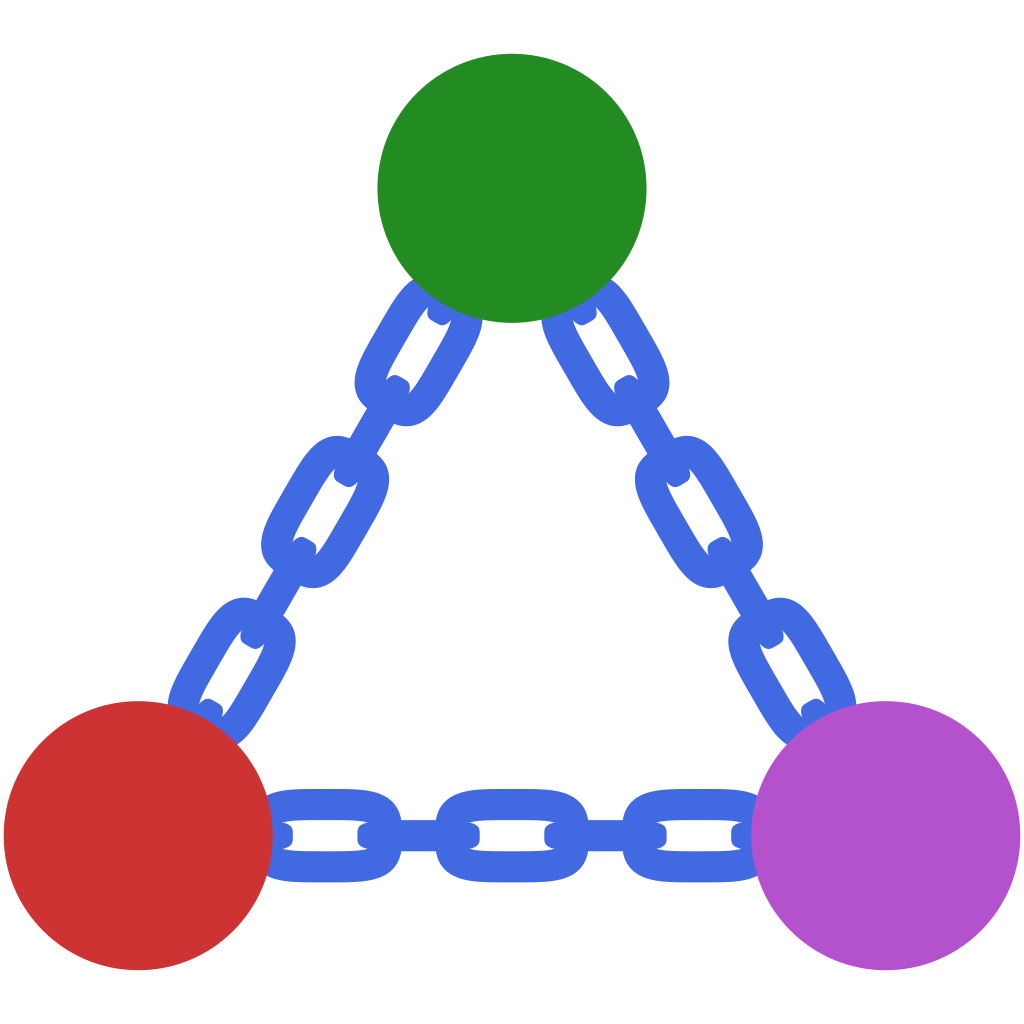
\includegraphics[width=5cm]{figs/juliaconstraints.png}}
  \caption{Logo of the \jc organization on GitHub that hosts, among other things, the \cnjl package.}
  \label{fig:juliaconstraints}
\end{figure}

On the other hand, Constraint-Based Local Search (\cbls) is a family of metaheuristics in which the neighborhood is constructed on the basis of an \emph{error function}, itself a quantitative representation of how far the current configuration is from an admissible solution. We refer to the corresponding problems as Error Function Satisfaction Problem (\efsp) and Error Function Optimization Problem (\efop). In the case of \cbls, this is computed as a function of the constraints which are not currently satisfied. Error functions may be derived from the constraint satisfaction problem structure, hand-coded, automatically acquired by some machine learning process, or constructed as a combination of these methods. It should be noted that, the best performing systems resort to hand-tuned error functions, as witness~\cite{DBLP:books/sp/18/CodognetMDA18}.

As illustrated by Figure~\ref{fig:landscape}, a well-designed error function helps in converging faster towards better-quality solutions.  It does, however, introduce an additional layer of complexity to the user.

\begin{figure*}[t]
  \centering
  \subcaptionbox{CSP landscape\label{sfig:csp}}{
    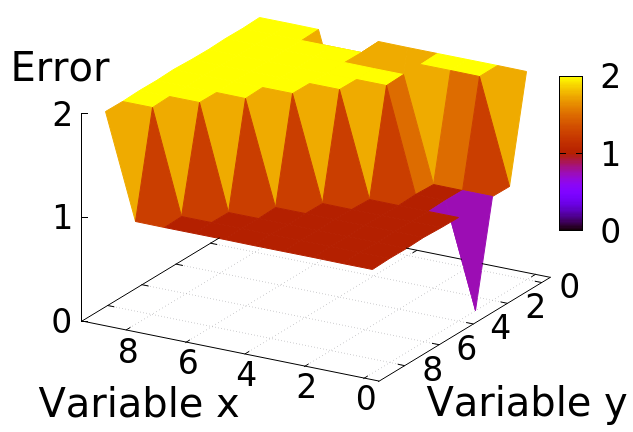
\includegraphics[width = .95\columnwidth]{figs/csp_landscape_complex_zero_big.png}
  }
  \hfill
  \subcaptionbox{EFSP landscape\label{sfig:efsp}}{
    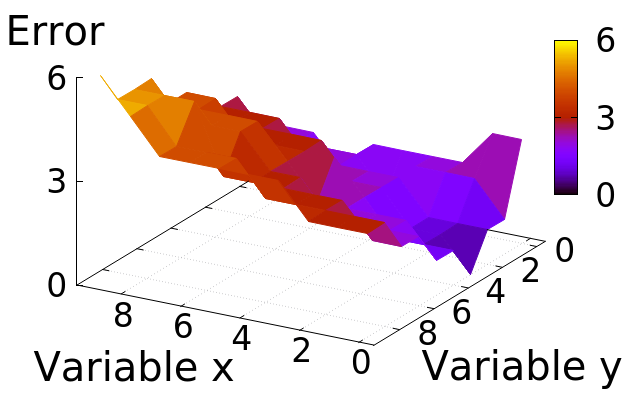
\includegraphics[width = .95\columnwidth]{figs/efsp_landscape_complex_zero_big.png}
  }\caption{
    Comparison of a Constraint Satisfaction Problem (CSP) and an Error
    Function Satisfaction Problem (\efsp) landscapes. The finer scale
    in the error heuristic of the \efsp leads to a better convergence
    rate.}\label{fig:landscape}
\end{figure*}

\subsection{Interpretable Compositional Networks (ICN)}
\label{subsec:icn}

In \cite{richoux2020automatic}, we proposed a neural network inspired by Compositional Pattern-Producing Networks (\cppn) to learn (highly) combinatorial functions as non-linear combinations of elementary operations. \(\cppn\)s~\cite{stanley2007cppn} are themselves a variant of artificial neural networks. While neurons in regular neural networks usually  contain sigmoid-like functions only (such  as ReLU, \ie{} Rectified Linear  Unit), \cppn's neurons can contain many other kinds of functions: sigmoids, Gaussians, trigonometric functions, and linear functions among others.
\(\cppn\)s are often used to generate 2D or 3D images by applying the function modeled by a \cppn giving each pixel individually as input, instead of considering all pixels at once. This simple trick allows the learned \cppn model to produce images of any resolution.

We propose our variant by taking these two principles from \cppn: having neurons containing one operation among many possible ones, and handling inputs in a size-independent fashion. Due to their interpretable nature, we named our variant \textbf{Interpretable Compositional Networks} (\icn).

Although ICNs are not limited to learning function for \efsp/\efop, the original structure was designed to learn compositions weighted in accordance to the hamming metric \cite{richoux2020automatic}. The hamming distance between a configuration and its closest solution is a meaningful indicator of the number of variables needed to be changed. Manhattan and other variants of minkowski comparison are other example of possible metrics.

An ICN is made of several layers of (possibly exclusive) operations such that the first layers accept a vector as input and the last layer returns a single numerical value. Generally, layers alter there input in three possible ways: \emph{increment}, \emph{decrement}, or \emph{conservation} of the dimension of the input.

\begin{figure}[t]
  \centerline{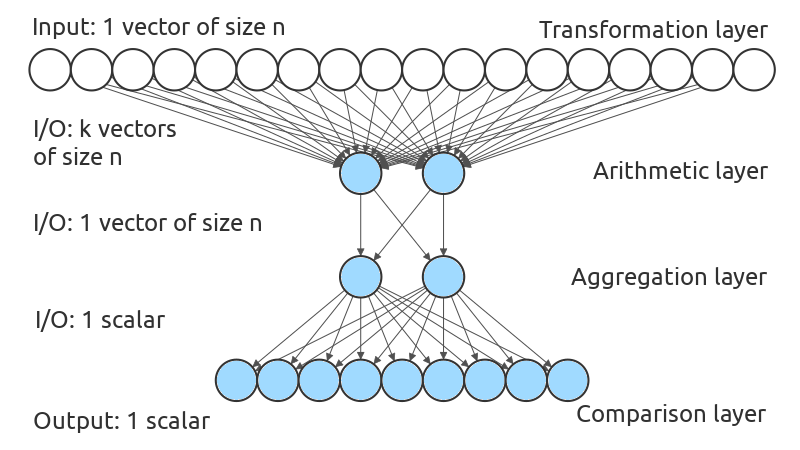
\includegraphics[width=\columnwidth]{figs/model_nn.png}}
  \caption{Scheme of the basic 4-layers ICN model used in \efsp/\efop. Layers with blue neurons have mutually exclusive operations. the \emph{transformation} layer increases the input dimension, the \emph{arithmetic} and \emph{aggregation} layers reduces it, and the \emph{comparison} layer leaves it untouched. The figure is taken from \cite{richoux2020automatic}.}
  \label{fig:model_icn}
\end{figure}

In the context of \efsp/\efop, the output should be non-negative if the constraint is violated and equal to 0 otherwise. As shown by Figure \ref{fig:model_icn}, our \(\icn\)s are
composed of four layers, each of them having a specific purpose and
themselves composed of neurons applying  a unique operation each.  All
neurons  from  a  layer  are  linked to  all  neurons  from  the  next
layer. The weight on each link is purely binary: its value is either 0
or 1. This restriction is  crucial to obtain interpretable functions. We refer the reader to \cite{richoux2020automatic} for a more comprehensive definition.

% \subsection{A first C++ library}
% \label{subsec:cplusplus}

In \cite{richoux2020automatic} we introduced the concept of ICN and a first implementation for Constraint Programming as a C++ library\footnote{\url{https://github.com/richoux/LearningUtilityFunctions}}. The results were evaluated through the GHOST C++ solver \cite{richoux2016ghost} and serve as a proof of concept that most of the models give scalable functions, and remain fairly effective using incomplete training sets.

As mentioned in Section \ref{sec:use}, \cnjl generates code for a direct use in Julia, but also exports usable code for both the GHOST(C++) and AdaptiveSearch (C)\footnote{This feature is a WIP at the moment this article is submitted, but is expected to be completed in the coming weeks.}. The code exported in C++, that is the \emph{operations} of each neuron, is strongly inspired by our C++ library.

This work is part of a collection of articles that introduce the theoretical background of ICN \cite{richoux2020automatic}, a user-friendly implementation in Julia, and an extensive collection of benchmarks \cite{baffier2022interpretable}.
Please note that the default parameters, and semi-automated learning parameters for advanced users, in \cnjl will improve along the results in \cite{baffier2022interpretable} computed from \icnbjl on an HPC cluster.

\begin{figure*}[t]
  \centerline{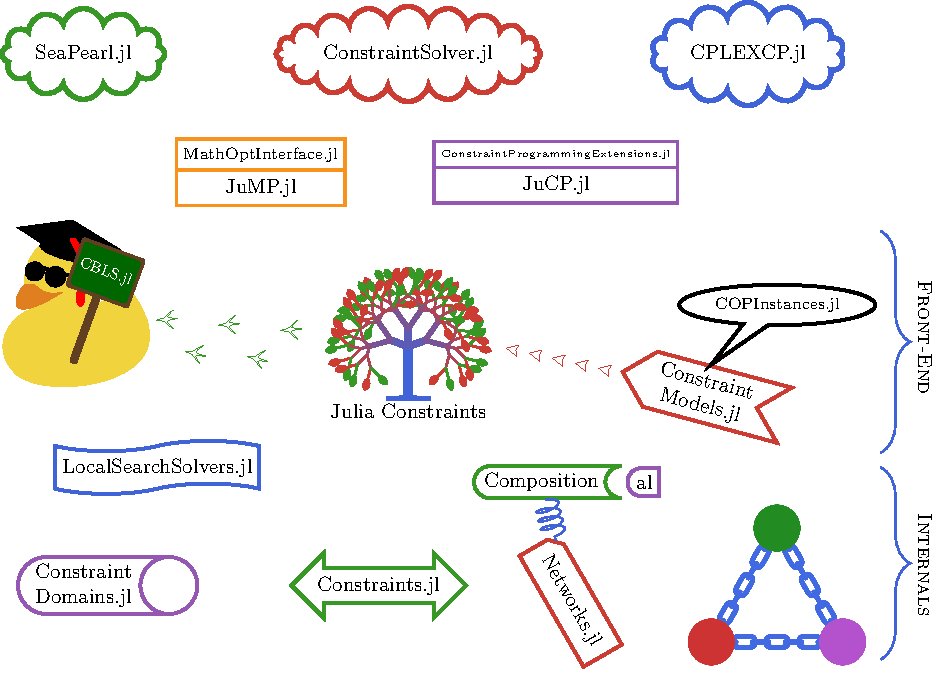
\includegraphics[page=1, width=.9\textwidth]{figs/overview.pdf}}
  \caption{Overview of the Constraint Programming ecosystem in Julia, including \jc. \emph{Front-End} and \emph{Internals} refer to the latest. Note that, at the moment of the writing, \texttt{ConstraintProgrammingExtension.jl}, \texttt{JuCP.jl}, and \texttt{COPInstances.jl} are temporary names.}
  \label{fig:overview}
\end{figure*}

\FloatBarrier

\section{The example of the \jc framework}
\label{sec:juliaconstraints}

The \cnjl package is part of the \jc GitHub organization that proposes a first collection of Julia packages for Constraint-Based Local Search (CBLS), a subfield of Constraint Programming. All packages fall under the MIT license.

The main goal of this framework is to provide a set of high level semi-automatic tools which strike a good compromise between efficiency and ease of modeling.

\subsection{History of \jc}
\label{subsec:history}

The \lssjl package is a Constraint-Based Local Search framework started in Fall 2020 and inspired by other CBLS solvers such as GHOST (C++) and AdaptiveSearch (C) that allows users to tune their own solver.

During the development of LocalSearchSolvers.jl, we decided to split the code and functionality of the original framework into several independent packages for ease of maintenance and in hopes of providing common tools for other constraint programming packages in Julia. These tools were collected into the \jc ecosystem.

The global state of the Constraint Programming ecosystem is presented in Figure \ref{fig:overview}. Beside the CBLS framework of \jc detailed below, other solvers are complete search methods, such as ConstraintSolver.jl\footnote{\url{https://github.com/Wikunia/ConstraintSolver.jl}}, CPLEXCP.jl\footnote{\url{https://github.com/dourouc05/CPLEXCP.jl}}, and SeaPearl.jl \cite{chalumeau2021seapearl}.

\paragraph*{State of the packages in \jc}

\begin{itemize}
  \item Stable packages
  \begin{itemize}
    \item \cnjl: internal tool to provide semi-automated error functions. Also, a standalone to learn compositions for combinatorial functions\footnote{At the time of submission, \cnjl is not yet release as \texttt{v1}. Some minor changes are expected from the results of the benchmarks in \cite{baffier2022interpretable} that will be submitted at the end of October.}
  \end{itemize}
  \item Beta packages (usable with frequent breaking changes)
  \begin{itemize}
    \item \cdjl: creation of discrete, continuous, and arbitrary domains
    \item \cjl: generation of constraints from a boolean concept or an error function. Also, list usual constraints and their properties
    \item \lssjl: A CBLS framework in Julia with built-in parallel and distributed scalability
    \item \cblsjl: A MOI/JuMP wrapper for LocalSearchSolvers
    \item \cmjl: list of CP models for \cblsjl and \lssjl
  \end{itemize}

\end{itemize}



\subsection{The \emph{JuMP} ecosystem} % 3-6p
\label{subsec:jump}

JuMP is a modeling language accessible through its main package
JuMP.jl \cite{DunningHuchetteLubin2017} and many supporting Julia packages. Beneath JuMP is an
abstraction layer called MathOptInterface
(MOI)~\cite{MathOptInterface-2021}. One can make a parallel
between MOI/JuMP and FlatZinc/MiniZinc~\cite{nethercote2007minizinc},
common modeling tools of the Constraint Programming community.
Recently, the
\href{https://github.com/dourouc05/ConstraintProgrammingExtensions.jl}{ConstraintProgrammingExtensions.jl}
package that extends MOI/JuMP to the Constraint Programming world was
made available. It is likely to become the recommended unified JuMP
modeling extension for the Julia Constraint Programming solvers.

\subsection{A simple example with \texttt{CBLS.jl}}
\label{subsec:example}

\begin{figure}[t]
  \centerline{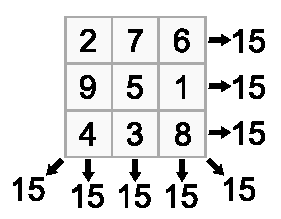
\includegraphics[page=1, width=.75\columnwidth]{figs/magicsquare.pdf}}
  \caption{A solved magic-square of size $3$. The \emph{magic sum} is equal to $15$. Image from Wikipedia's user \textsc{Phidauex}.}
  \label{fig:magicsquare}
\end{figure}

Our CBLS framework uses three levels of modeling syntax: a \emph{raw} Julia syntax, and both MOI and JuMP syntaxes. In this article, we will only use the highest level one, the JuMP syntax.

A Magic Square of order $n$ is composed of $n^2$ distinct values ranging from $1$ to $n^2$ layed out as a square array $X$.  These values need to be arranged such that the sums of each diagonal, row and column be equal to the same value, the magic sum $\Sigma$.

\[ \sum_{j=1}^{n} X_{ij} = \sum_{i=1}^{n} X_{ij} = \sum_{j=1}^{n} X_{ii} = \sum_{j=1}^{n} X_{i,n-i+1} = \frac{n(n^{2}+1)}{2} = \Sigma \]

In \cmjl, we use the following code to generate a magic-square instance.

\begin{lstlisting}[language = Julia]
# Import CBLS.jl and JuMP.jl
using CBLS, JuMP

function magic_square(n::Integer)
model = Model(CBLS.Optimizer)
N = n^2
Σ = n * (N + 1) / 2
@variable(model, 1 <= X[1:n, 1:n] <= N, Int)
@constraint(model, vec(X) in AllDifferent())
for i in 1:n
  @constraint(model, X[i,:] in Linear(Σ))
  @constraint(model, X[:,i] in Linear(Σ))
end
@constraint(model,
  [X[i,i] for i in 1:n] in Linear(Σ)
)
@constraint(model,
  [X[i,n+1-i] for i in 1:n] in Linear(Σ)
)
  return model, X
end
\end{lstlisting}

\section{A flexible implementation}
\label{sec:implementation}

As mentioned in Subsection \ref{subsec:icn}, \cnjl extends the work of the first C++ library used for prototyping in \cite{richoux2020automatic}. We decided to use some features of the Julia language to ease provisioning flexibility and broader features to ICNs.

\subsection{The Julia language}
\label{subsec:julialang}

The Julia language was introduced in~\cite{bezanson2017julia} and
purports to be a new take on \emph{mathematical programming}.  Some
key features of the language, according to the official website, which
led us to consider it as an implementation vehicle:
\begin{description}
\item[Fast:] Julia was designed from the beginning for high
  performance.  Julia programs compile to efficient native code for
  multiple platforms via LLVM~\cite{lattner2004llvm}.
\item[Dynamic:] It is dynamically typed, feels like a scripting
  language, and has good support for interactive use.
\item[Reproducible:] Reproducible environments make it possible to
  recreate the same Julia environment every time, across platforms,
  with pre-built binaries.
\item[Composable:] It uses multiple dispatch as a paradigm, making it
  easy to express many object-oriented and functional programming
  patterns.
\item[General-purpose:] It provides metaprogramming, asynchronous I/O,
  debugging, logging, profiling, a package manager, and more.  One can
  build entire Applications and Microservices in Julia.
\item[Open source:] It is an open source project with over 1,000
  contributors.  It is made available under the MIT license and the
  source code is available on GitHub.
\end{description}

\subsection{Layers of operations}
\label{subsec:layers}

A layer is defined by a non-empty collection of (possibly mutually exclusive) operations. Our basic ICN (for \efsp/\efop) is composed of four layers: \emph{transformation}, \emph{arithmetic} (exclusive), \emph{aggregation} (exclusive), and \emph{comparison} (exclusive). An illustration is given as Figure \ref{fig:model_icn}. The \texttt{Layer} structure stores these operations.

\begin{lstlisting}[language = Julia]
struct Layer
  functions::LittleDict{Symbol, Function}
  exclusive::Bool
end
\end{lstlisting}

The most complex layer is probably the \emph{transformation} layer. An operation (neuron) of this layer is defined over a vector of values and an optional parameter. As it is often simpler to define a transformation as a function over a specific index of the input vector, we provide meta-programming utility functions to generate vectorized methods: \texttt{lazy} and \texttt{lazy\_param}.

\begin{lstlisting}[language = Julia]
# Transformation defined for a vector
tr_identity(x; param=nothing) = identity(x)

# Transformation defined for the index of a vector
tr_count_eq(i, x; param=nothing) =
  count(y -> x[i] == y, x) - 1
tr_count_eq_param(i, x; param) =
  count(y -> y == x[i] + param, x)

# Generating vectorized versions
lazy(tr_count_eq)
lazy_param(tr_count_eq_param)
\end{lstlisting}

When a concept is provided to an ICN, the user can provide an optional parameter input with the keyword argument \texttt{param}. A layer will be generated with or without the parametric operations (neurons) based on \texttt{param}'s value. Follow a shortened version of the transformation layer generator.

\begin{lstlisting}[language = Julia]
function transformation_layer(param=false)
  transformations = LittleDict{Symbol,Function}(
    :identity => tr_identity,
    :count_eq => tr_count_eq,
    # ...
  )
  if param
    tr_param = LittleDict{Symbol, Function}(
      :count_eq_param => tr_count_eq_param,
      # ...
    )
    transformations = LittleDict(
      union(transformations, tr_param)
    )
  end
  return Layer(transformations, false)
end
\end{lstlisting}

All methods required for the definition of additional layers are all available. An (unweighted) ICN is simply generated from a sequence of layers. After a learning phase using the a genetic algorithm from \texttt{Evolutionary.jl}\footnote{\url{https://github.com/wildart/Evolutionary.jl}}, this ICN can output a composition in various forms.

\subsection{Composition}
\label{subsec:composition}

Once the ICN is weighted, we store its  output as a composition with three forms.
A collection of \texttt{Symbol}s per layer of the ICN that allows the generation of code as a pre-process in any language, assuming the operations encoding in that language are available. \cnjl currently supports Julia, C, and C++.

A composition also stores a Julia object of type \texttt{Function} to apply the composition in a dynamic fashion.

\begin{lstlisting}[language = Julia]
struct Composition{F<:Function}
  code::Dict{Symbol,String}
  f::F
  symbols::Vector{Vector{Symbol}}
end
\end{lstlisting}

As mentioned above, an ICN outputs a composition, \ie{} a mathematical function composed of several basic operations. The \texttt{code} function returns the definition of a composition in either a mathematical or a programming language. From \texttt{v1} of \cnjl, \texttt{code} accepts \texttt{:maths} (default), \texttt{:Julia}, \texttt{:C}, \texttt{:Cpp} as values for the \texttt{lang} keyword argument.

\begin{lstlisting}[language = Julia]
function code(
  c::Composition, lang=:maths;
  name="composition"
)
  return get!(
    c.code, lang, generate(c, name, Val(lang))
  )
end
\end{lstlisting}

\section{How to use \cnjl}
\label{sec:use}

This section covers the essential steps to use ICN in a Julia environment. The actions required are few, which allow users to apply or export compositions effortlessly.

\subsection{Installation and import}
\label{subsec:install}

\cnjl will keep compatibility with the latest stable and LTS releases of Julia\footnote{Note that at the time of writing, Julia has just released \texttt{v1.7}. Compatibility with last LTS will start from the next LTS release.}. We recommend the users to install the latest version of Julia\footnote{\url{https://julialang.org/downloads/}} and to call it with \texttt{julia -t auto} which launch Julia with all available threads on the local machine. Installing \cnjl from the Julia REPL is as simple as:

\begin{lstlisting}[language = Julia]
using Pkg
Pkg.update()
Pkg.add("CompositionalNetworks")
\end{lstlisting}

Alternatively, one can install from the package REPL (simply press `]' in a Julia session) in a single command.

\begin{lstlisting}
add CompositionalNetworks
\end{lstlisting}

Finally, loading the package is done by calling:
\begin{lstlisting}[language = Julia]
using CompositionalNetworks
\end{lstlisting}

Note that from Julia \texttt{v1.7}, calling \texttt{using} on uninstalled package will prompt the user to install it. Hence, the last command is the only one strictly required.

\subsection{Explore, learn, and compose}
\label{subsec:xlc}

It is far from practical to apply the internals of \cnjl step-by-step. We provide a user-friendly sequence of higher-level actions that fits most of expected uses of this package:
\begin{itemize}
  \item \emph{explore} a search space according to a collection of variables domains, a metric, and a concept with an optional parameter
  \item \emph{learn} the weights of an ICN on that space according to the same metric
  \item \emph{compose} the elementary operations according to the weights of the ICN
\end{itemize}

The whole sequence can be executed through \texttt{explore\_learn\_compose}. That function accepts an increasingly large collection of (keyword) arguments:
\begin{itemize}
  \item \texttt{domains}: domains of the variables that define the training space
  \item \texttt{concept}: the concept of the targeted constraint
  \item \texttt{param}: an optional parameter of the constraint
  \item \texttt{search}: either \texttt{:flexible},\texttt{:partial} or \texttt{:complete} search. Flexible search will use \texttt{search\_limit} and \texttt{solutions\_limit} to determine if the search space needs to be partially or completely explored
  \item \texttt{global\_iter}: number of learning iterations
  \item \texttt{local\_iter}: number of generations in the underlying genetic algorithm
  \item \texttt{metric}: the metric to measure the distance between a configuration and known solutions
  \item \texttt{pop\_size}: size of the population in the genetic algorithm
  \item \texttt{complete\_search\_limit}: used in conjunction with \texttt{solution\_limit} to determine if a flexible search is set to complete or partial
  \item \texttt{solutions\_limit}: see above
  \item \texttt{sampler}: optional sampler function for a collection of configurations
  \item \texttt{configurations}: optional collection of configurations to use as a training set
  \item \texttt{memoize}: if true, use a memoized version of the metric
\end{itemize}
Each of those actions is semi-automated through default parameters and machine learning over a large collection of benchmarks \cite{baffier2022interpretable}.

\begin{lstlisting}[language = Julia]
function explore_learn_compose(
  domains,
  concept,
  param=nothing;
  global_iter=Threads.nthreads(),
  local_iter=100,
  metric=:hamming,
  pop_size=400,
  search=:flexible,
  complete_search_limit=1000,
  solutions_limit=100,
  sampler=nothing,
  configurations=explore(
    domains, concept, param;
    search, complete_search_limit, solutions_limit
  ),
  memoize=true,
)
  dom_size = maximum(domain_size, domains)
  solutions, non_sltns = configurations
  return learn_compose(
    solutions,
    non_sltns,
    dom_size,
    param;
    local_iter,
    global_iter,
    metric,
    pop_size,
    sampler,
    memoize,
  )
end
\end{lstlisting}

A long-term goal of \cnjl is to make the three first arguments optional too. We hope that such improvement will be used within \jc, for instance within the following more advanced examples.

\subsection{Advanced examples}
\label{subsec:advanced}

Large scale use of \cnjl is made within \jc and appears in:
\begin{itemize}
  \item \cjl: the learning script can be found in \texttt{/src/learn.jl} and can be called as \texttt{learn\_from\_icn()}.
  \item \icnbjl: an extensive collection of ICN benchmarks run on an HPC cluster. This package is not registered in the general registry of Julia packages.
\end{itemize}

\section{Future challenges}
\label{sec:future}

We envisage several directions for future improvement of ICN within \cnjl. Follows a non-comprehensive list of the most challenging features.

\paragraph*{New operations in existing layers} As the experiments have shown in \cite{richoux2020automatic,baffier2022interpretable}, some concepts are too complex to be covered with the current set of operations. The most direct solutions is to provide a broader collection of elementary operations.

\paragraph*{New layers} Applied to \efsp/\efop or not, it is likely that adding some layers of operation could cover a wider spectrum of combinatorial functions (with some cost for the interpretability and computation time).

\paragraph*{Reinforcement learning} Some limitations in the ICN parametrization and metrics could be solved at runtime with dynamic learning. In the \jc context, this could occur at the solver execution.

\paragraph*{Apply ICN to other fields and problems} Contributions and suggestions are more than welcome!

\section{Problems, constraints, and compositions zoo}
\label{sec:zoo}

The problems modelled, and the compositions extracted in this section are subject to future changes and improvements of the JuMP/JuCP packages. However, the keys ideas are presented here and examples will be updated accordingly within \jc in the future. We welcome GitHub issues and pull requests.

\subsection{A few combinatorial models}
\label{subsec:models}

At the moment, \cmjl hosts more than a dozen models. Along with \emph{Magic Square} introduced in Section \ref{subsec:example}, we present models for two other classical optimization problems: \emph{Golomb ruler} and \emph{minimum cut}. The choice was made to cover different type of constraints, with error functions learned from \cnjl.

Note that a model for the minimum cut problem in a network requires a matrix (graph) as input. Additionally, we add the optional argument of the interdiction of some links in the cut, which lead to an intractable problem called \emph{Network Interdiction} \cite{baffier2016parametric}.


\begin{lstlisting}[language = Julia]
function mincut(graph, source, sink, interdiction)
  m = JuMP.Model(CBLS.Optimizer)
  n = size(graph, 1)
  separator = n + 1

  @variable(m, 0 <= X[1:separator] <= n, Int)

  @constraint(m,
    [X[source], X[separator], X[sink]] in Ordered()
  )
  @constraint(m, X in AllDifferent())

  obj(x...) = o_mincut(graph, x...; interdiction)
  @objective(m, Min, ScalarFunction(obj))

  return m, X
end
\end{lstlisting}

In contrast, an instance of the Golomb ruler problem does not require specific dataset. However, this problem exists as both satisfaction and optimization variants.

\begin{lstlisting}[language = Julia]
function golomb(n, L)
  m = JuMP.Model(CBLS.Optimizer)

  @variable(m, 0 <= X[1:n] <= L, Int)

  @constraint(m, X in AllDifferent())

  # optional for output readability
  @constraint(m, X in Ordered())

  # No two pairs have the same length
  for i in 1:(n - 1), j in (i + 1):n
    for k in i:(n - 1), l in (k + 1):n
      (i, j) < (k, l) || continue
      @constraint(m,
        [X[i], X[j], X[k], X[l]] in DistDifferent()
      )
    end
  end

  # Add objective
  @objective(m, Min, ScalarFunction(maximum))

  return m, X
end
\end{lstlisting}

\subsection{Constraints and compositions}
\label{subsec:constraints}

Along with the magic-square model in Section \ref{sec:introduction}, the models in this zoo use the following constraints: \texttt{:all\_different}, \texttt{:dist\_different}, \texttt{:linear}, and \texttt{:ordered}\footnote{The code provided here will be updated following the results of the benchmark in \cite{baffier2022interpretable}. In particular, for \texttt{:dist\_different} and \texttt{:linear}, the current code is a hand-written function.}.\newline

The \emph{AllDifferent} constraint ensures that all the values of a given configuration are unique.

\begin{lstlisting}[language = Julia]
function all_different(x;
  X = zeros(length(x), 1), param=nothing, dom_size
)
  tr_in(Tuple([tr_count_eq_left]), X, x, param)
  for i in 1:length(x)
    X[i,1] = ar_sum(@view X[i,:])
  end
  return ag_count_positive(@view X[:,1]) |> (
      y -> co_identity(
        y; param, dom_size, nvars=length(x)
      )
    )
end
\end{lstlisting}

\emph{DistDifferent} is constraint ensuring that \(|x[1] - x[2]| \neq |x[3] - x[4]|\) for any vector $x$ of size $4$.

\begin{lstlisting}[language = Julia]
function dist_different(x)
  return abs(x[1] - x[2]) != abs(x[3] - x[4])
end
\end{lstlisting}

\emph{Linear} (also called \emph{Sum} or \emph{LinearSum} in the literature) Global ensures that the sum of the values of $x$ is equal to a given parameter $param$. Note that this version is a simplification of a linear sum of values with some coefficients.

\begin{lstlisting}[language = Julia]
function linear(x; param, dom_size)
  return abs(sum(x) - param) / dom_size
end
\end{lstlisting}

\emph{Ordered} is a constraint ensuring that all the values of $x$ are ordered (here in a decreasing order).

\begin{lstlisting}[language = Julia]
function ordered(x;
  X = zeros(length(x), 1), param=nothing, dom_size
)
  tr_in(
    Tuple([tr_contiguous_vals_minus]), X, x, param
  )
  for i in 1:length(x)
    X[i,1] = ar_sum(@view X[i,:])
  end
  return ag_count_positive(@view X[:,1]) |> (
      y -> co_identity(
        y; param, dom_size, nvars=length(x)
      )
    )
end
\end{lstlisting}

\section{Acknowledgements}
\label{sec:acknowledgements}

We're grateful to Ricardo \textsc{Rosa} and Pranshu \textsc{Malik} for the logo of \jc presented as Figure \ref{fig:juliaconstraints}.

% **************GENERATED FILE, DO NOT EDIT**************

\bibliographystyle{juliacon}
\bibliography{ref.bib}


\end{document}

% Inspired by the International Journal of Computer Applications template
